
%%%%%%%%%%%%%%%%%%%%%%% file typeinst.tex %%%%%%%%%%%%%%%%%%%%%%%%%
%
% This is the LaTeX source for the instructions to authors using
% the LaTeX document class 'llncs.cls' for contributions to
% the Lecture Notes in Computer Sciences series.
% http://www.springer.com/lncs       Springer Heidelberg 2006/05/04
%
% It may be used as a template for your own input - copy it
% to a new file with a new name and use it as the basis
% for your article.
%
% NB: the document class 'llncs' has its own and detailed documentation, see
% ftp://ftp.springer.de/data/pubftp/pub/tex/latex/llncs/latex2e/llncsdoc.pdf
%
%%%%%%%%%%%%%%%%%%%%%%%%%%%%%%%%%%%%%%%%%%%%%%%%%%%%%%%%%%%%%%%%%%%


\documentclass[runningheads,a4paper]{llncs}

\usepackage[english, spanish]{babel}
\usepackage[utf8]{inputenc}
\usepackage[T1]{fontenc}
\usepackage{lmodern}
\usepackage{amssymb}
\setcounter{tocdepth}{3}
\usepackage{graphicx}
\usepackage{epstopdf}
\usepackage{float}

\usepackage{url}

\newcommand{\keywords}[1]{\par\addvspace\baselineskip
\noindent\keywordname\enspace\ignorespaces#1}

 \setcounter{secnumdepth}{3}

\begin{document}

\mainmatter  % start of an individual contribution

% first the title is needed
\title{Algoritmos de Búsqueda Basados en Trayectorias.}

% a short form should be given in case it is too long for the running head
\titlerunning{Algoritmos de Búsqueda Basados en Trayectorias.}

% the name(s) of the author(s) follow(s) next
%
% NB: Chinese authors should write their first names(s) in front of
% their surnames. This ensures that the names appear correctly in
% the running heads and the author index.
%
\author{Alejandro Trujillo Caballero
}
%
\authorrunning{Algoritmos de Búsqueda Basados en Trayectorias..}
% (feature abused for this document to repeat the title also on left hand pages)

% the affiliations are given next; don't give your e-mail address
% unless you accept that it will be published
\institute{Universidad de Huelva. Grado en Ingeniería Informática.}

%
% NB: a more complex sample for affiliations and the mapping to the
% corresponding authors can be found in the file "llncs.dem"
% (search for the string "\mainmatter" where a contribution starts).
% "llncs.dem" accompanies the document class "llncs.cls".
%

\toctitle{Proceso KDD Completo}
\tocauthor{Alejandro Trujillo Caballero}
\maketitle

\selectlanguage{spanish}
\begin{abstract}
Análisis del funcionamiento de varios algoritmos de búsqueda (Aleatoria, Local, Enfriamiento Simulado, Tabú y Greedy) aplicados al Problema de Asignación Cuadrática.
\keywords{Búsqueda, Búsqueda Local, Búsqueda Aleatoria, Enfriamiento Simulado, Búsqueda Tabú, Greedy, Asignación Cuadrática (QAP).}
\end{abstract}


\section{Introducción}

\subsection{Problema de Asignación Cuadrática}

El Problema de Asignación Cuadrática (QAP) es un problema de optimización combinatoria que consiste en asignar una serie de unidades a localizaciones (teniendo el mismo número de ambas). El objetivo es optimizar una función de coste que consiste en la suma de los productos de la distancia entre localizaciones y el transito entre las unidades asignadas.


 Un ejemplo de aplicación de este problema podría ser la distribución de los diferentes departamentos de un hospital en las diferentes plantas o zonas del edificio.

Para analizar el funcionamiento de los diferentes algoritmos se han utilizado tres ejemplos de diferente tamaño de los cuales se conoce el coste de la solución óptima:

\begin{itemize}
\item \textbf{Tai25b:} 25 lugares y unidades, coste: 344355646.
\item \textbf{Sko90:} 90 lugares y unidades, coste: 115534.
\item \textbf{Tai150b:} 150 lugares y unidades, coste: 498896643.
\end{itemize}

\section{Algoritmos Analizados}

\subsection{Algoritmo Greedy o Voraz}

Se ha utilizado un algoritmo voraz como base para el análisis del resto de algoritmos.

El algoritmo intenta minimizar el coste asignado las unidades con mayor transito a las localizaciones más céntricas.

El algoritmo siempre sigue el mismo criterio para construir una solución y obtiene la misma por lo que no puede considerase una búsqueda.

\subsection{Búsqueda Aleatoria}

El algoritmo de Búsqueda Aleatoria es la búsqueda más simple de las estudiadas.

En cada iteración se genera una solución aleatoria al problema y se calcula su coste. Tras un número de iteraciones fijas se devuelve la mejor solución (la de menor coste) entre todas las analizadas.

Para nuestro estudio, se han realizado 1600*n iteraciones en cada ejecución donde n es la dimensión del problema (número de localizaciones/unidades).

\subsection{Búsquedas Basadas en Vecindad}

Los tres algoritmos restantes funcionan en torno al concepto de solución vecina. Para el problema QAP se ha considerado que dos soluciones son vecinas si puede obtenerse una a partir de la otra intercambiando únicamente dos parejas localización-unidad, asignando la unidad de la primera a la localización de la segunda y viceversa.

\subsubsection{Búsqueda Local}
~\\

La Búsqueda Local parte de una solución aleatoria y en cada iteración estudia los vecinos de la solución en busca de una mejor (que estudiará en la siguiente iteración). 

Este algoritmo base puede especificarse para obtener diferentes implementaciones en función de diferentes parámetros:

\begin{itemize}
\item \textbf{Número de Vecinos}: Puede variarse el número de vecinos que se estudian en cada iteración, ya sea utilizando un número fijo, analizando todos los vecinos posibles, analizando hasta encontrar uno que mejore al actual, etc...
\item \textbf{Criterio de Parada:} El algoritmo puede detenerse cuando ya no encuentre ningún vecino mejor, puede ejecutarse un número de iteraciones fijo o puede utilizarse orto criterio más complejo.
\end{itemize} 

En nuestro caso, analizamos en cada iteración todos los vecinos posibles buscando el mejor de ellos y  el algoritmo se detiene cuando en una iteración no existe un vecino que mejore la solución, obteniéndose como resultado la solución que se analiza en ese momento.

\subsubsection{Enfriamiento Simulado}
~\\

El algoritmo de Enfriamiento Simulado funciona como la Búsqueda Local pero añadiendo la posibilidad de aceptar soluciones que empeoren a la actual de forma que la búsqueda pueda escapar de mínimos locales.

Para ello utiliza el concepto de temperatura, cuando la temperatura es alta la probabilidad de aceptar una solución peor que la actual es mayor (al igual que en un gas a alta temperatura es más probable que una partícula escape de un pozo de potencial) y conforme el algoritmo avanza la temperatura va disminuyendo (el sistema se enfría).

El algoritmo utilizado tiene las siguientes características:

\begin{itemize}
\item \textbf{Solución inicial: } Se parte de una solución Greedy.
\item \textbf{Temperatura Inicial:} Se obtiene aplicando:  
\begin{equation}
T_0 = \frac{\mu}{-log(\phi)} C(S_i) 
\end{equation}
Donde C es la función de coste, $S_i$ es la solución inicial, $\phi$ es la probabilidad de aceptar una solución un $\mu$ por 1 peor que la inicial y $\phi = \mu = 0.3$.

\item \textbf{Enfriamiento: } Cada iteración del algoritmo analiza un número fijo de vecinos (en nuestro caso 50) y se enfria siguiendo el esquema de Cauchy:
\begin{equation}
T_k = T_0 / (1 + k)
\end{equation}
Donde k es la iteración actual.
\item \textbf{Condición de parada: } El algoritmo se detendrá tras un número máximo de iteraciones (en nuestro caso 80*n).
\end{itemize}

\subsubsection{Búsqueda Tabú}
~\\
La Búsqueda Tabú añade dos mecánicas a la busqueda local para mejorar los resultados:

\begin{itemize}
\item \textbf{Memoria: } Utiliza dos tipos de memoria para dirigir la ejecución del algoritmo: A corto plazo en forma de ``lista tabú'' que se utiliza para no repetir movimientos realizados recientemente al analizar nuevos vecinos y a largo plazo para guardar información de soluciones que dieron buenos o malos resultados.
\item \textbf{Reinicialización: } Este algoritmo añade la posibilidad de reiniciar la búsqueda bajo determinadas condiciones (un punto muerto, empeoramiento de los resultados...) 
\end{itemize}

La implementación realizada cumple las siguientes características: 

\begin{itemize}
\item \textbf{Solución Inicial: } El algoritmo parte de una solución Greedy.
\item \textbf{Criterios Tabú: } De cada solución analizada se guardan las asignaciones que la generaron y se prohíben soluciones nuevas que contengan alguna de esas asignaciones. Estos criterios se ignoran si la solución tiene menor coste que cualquiera encontrada hasta el momento. Inicialmente la lista tiene un tamaño de n/2 y funciona de forma circular.
\item \textbf{Análisis de Vecindad: } En cada iteración se analizan 40 vecinos y se selecciona el mejor que cumpla los criterios tabú.
\item \textbf{Criterios de parada y reinicialización: } El algoritmo ejecuta 40*n iteraciones y realiza una reinicialización cada 8*n iteraciones (4 en total).
\item \textbf{Método de reinicialización: } En cada de reinicio, hay una probabilidad del 25\% de reiniciar usando una solución aleatoria, otro 25\% de reiniciar desde la mejor solución obtenida y un 50\% de reiniciar una solución mediante la memoria a largo plazo. Además en cada reinicio la lista tabú puede aumentar o disminuir su tamaño un 50\% con una probabilidad del 50\% cada caso.
\item \textbf{Memoria a largo plazo: } La memoria guarda los intercambios que se realizan par generar cada vecino aceptado por el algoritmo y llegado el caso se utiliza para generar una solución poco frecuente en una reinicialización asignando unidades a posiciones que han ocupado en pocas ocasiones.

\end{itemize}

\newpage
\section{Resultados}

Para analizar los algoritmos se han realizado 10 ejecuciones de cada uno con diferentes semillas para el generador de números aleatorios (ya que todos los algoritmos tiene algún componente aleatorio). 

A continuación se detallan los resultados obtenidos por cada algoritmo.


\begin{table}[H]
\centering
\caption{Costes de las soluciones proporcionadas por el algoritmo de Búsqueda Aleatoria}

\begin{tabular}{c || r | r | r }
Seed & \qquad  tai25 \qquad \quad & \qquad sko90 \qquad & \qquad \qquad tai150 \qquad\\\hline 
1 	& 1173664963 & 142420 & 683423057 \\
2	& 1194390165 & 141814 & 682175843 \\
3	& 1196021141 & 142056 & 682400410 \\
4	& 1201615718 & 141968 & 682907768 \\
5	& 1186447299 & 142246 & 682840264 \\
6	& 1224953864 & 142340 & 683620162 \\
7	& 1178951674 & 142506 & 681266728 \\
8	& 1194823852 & 141922 & 680849383 \\
9	& 1194916409 & 141802 & 681370190 \\
10	& 1199973625 & 141932 & 681353354 \\ \hline \hline
Media & 1194575871 & 142101 & 682220716 \\
Desv. T & 13949407 & 257 & 975284\\
\end{tabular}
\end{table}


\begin{table}[H]
\centering
\caption{Costes de las soluciones proporcionadas por el algoritmo de Búsqueda Local}

\begin{tabular}{c || r | r | r }
Seed & \qquad  tai25 \qquad \quad & \qquad sko90 \qquad & \qquad \qquad tai150 \qquad\\\hline 
1 	& 413373879 & 118426 & 517754022   \\
2	& 454985757 & 117582 & 513947464 		\\
3	& 353465428 & 118702 & 518922684 	\\
4	& 376336066 & 117696 & 520330467 	\\
5	& 411644796 & 118684 & 522055451 	\\
6	& 352048709 & 119516 & 520584440	\\
7	& 398432882 & 117446 & 515304984 	\\
8	& 472936529 & 118182 & 513041392 \\
9	& 459297404 & 119054 & 515305032 \\
10	& 422745919 & 119124 & 519625414 	\\ \hline \hline
Media & 411526737 & 118441 & 517687135\\
Desv. T &42674173 & 705 & 3103204\\
\end{tabular}
\end{table}


\begin{table}[H]
\centering
\caption{Costes de las soluciones proporcionadas por el algoritmo de Enfriamiento Simulado}

\begin{tabular}{c || r | r | r }
Seed & \qquad  tai25 \qquad \quad & \qquad sko90 \qquad & \qquad \qquad tai150 \qquad\\\hline 
1 	& 366621015 & 117626 & 513226444 \\
2	& 371725572 & 117552 & 513322732 \\
3	& 367818611 & 117170 & 514686453 \\
4	& 398264229 & 117824 & 517801729 \\
5	& 416599460 & 117956 & 515247819 \\
6	& 439006905 & 117568 & 515793920 \\
7	& 365491673 & 118028 & 514295612 \\
8	& 406671691 & 118298 & 519586022 \\
9	& 426523708 & 118000 & 524200812 \\
10	& 359474161 & 117208 & 515421269\\ \hline \hline
Media & 391819703 & 117723 & 516358281\\
Desv. T & 29176378 & 365 & 3374897\\
\end{tabular}
\end{table}

\begin{table}[H]
\centering
\caption{Costes de las soluciones proporcionadas por el algoritmo de Búsqueda Tabú}

\begin{tabular}{c || r | r | r }
Seed & \qquad  tai25 \qquad \quad & \qquad sko90 \qquad & \qquad \qquad tai150 \qquad\\\hline 
1 	& 344743823 & 118244 & 512796581 \\
2	& 345675295 & 117972 & 511883040 \\
3	& 395351036 & 117638 & 517545690 \\
4	& 347720408 & 117906 & 512090462 \\
5	& 363961225 & 118210 & 511258562 \\
6	& 346703840 & 117876 & 510626132 \\
7	& 347984063 & 117642 & 512807837 \\
8	& 347684843 & 118342 & 514336213 \\
9	& 346483036 & 118188 & 514097120 \\
10	& 364427055 & 118520 & 511212655\\ \hline \hline
Media & 355073462 & 118054 & 512865429  \\
Desv. T & 15939318 & 295 & 2040887 \\
\end{tabular}
\end{table}

\newpage
\subsection{Comparación de resultados}

\begin{table}[H]
\centering
\caption{Resultados globales de los algoritmos para el problema Tai25}
\begin{tabular}{c || r | r | r | r}
Algoritmo 	& Peor & Media & Mejor & Desv. T. \\ \hline
Óptimo 		& - 	& 344355646	&	-	&	-		\\
Greedy 		& - 	& 734935031	&	-	&	-		\\ \hline
B. Aleatoria &\quad  1224953864 & \quad  1194575871 & \quad 1173664963 & \quad \textbf{13949407} \\
B. Local & 472936529 & 411526737 & 352048709 & 42674173 \\
Enf. Simu & 439006905 & 391819703 & 359474161 & 29176378 \\
B. Tabú & \textbf{395351036} & \textbf{355073462} & \textbf{344743823} & 15939318 \\
\end{tabular}
\end{table}

\begin{figure}[H]
\center
\centerline{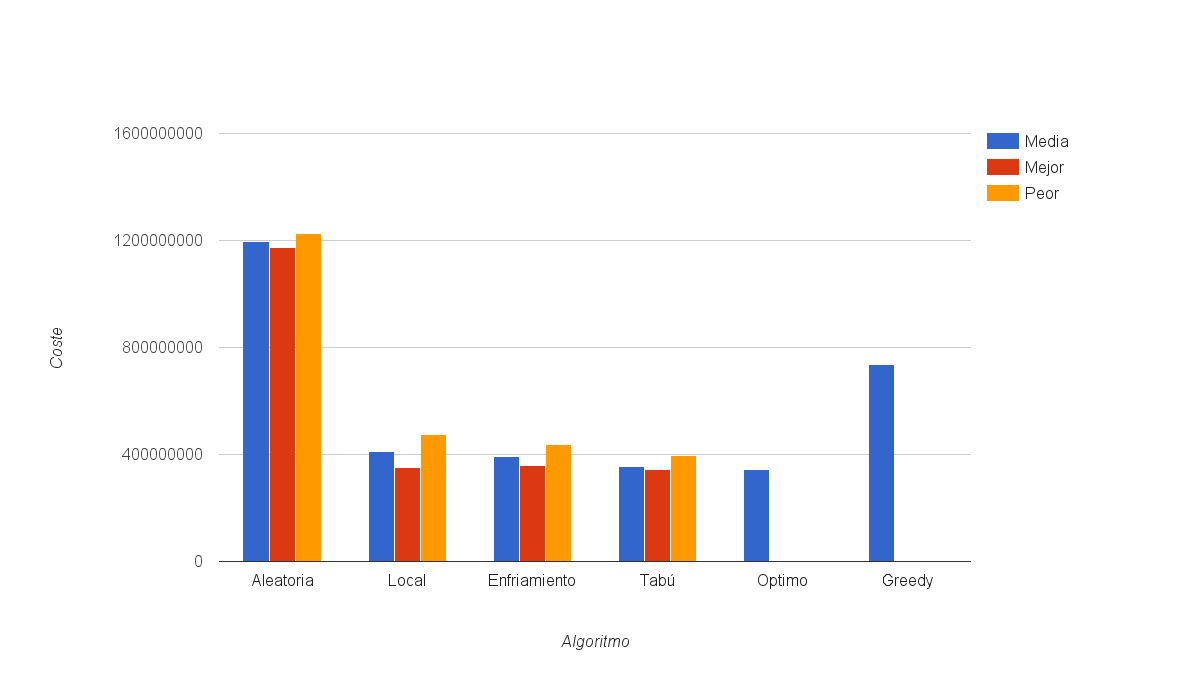
\includegraphics[scale=0.38]{./Grafico25.png}}
\caption{Resultados de los algoritmos para el problema Tai25}
\end{figure}

\begin{table}[H]
\centering
\caption{Resultados globales de los algoritmos para el problema Sko90}
\begin{tabular}{c || r | r | r | r}
Algoritmo 	& Peor & Media & Mejor & Desv. T. \\ \hline
Óptimo 		& - 	& 115534	&	-	&	-		\\
Greedy 		& - 	& 131262	&	-	&	-		\\ \hline
B. Aleatoria & \quad 142506 & \quad 142101 & \quad 141802 & \textbf{257} \\
B. Local & 119516 & 118441 & 117446 & 705 \\
Enf. Simu & \textbf{118298} & \textbf{117723} & \textbf{117170} & 365 \\
B. Tabú & 118520 & 118054 & 117638 & 295 \\
\end{tabular}
\end{table}


\begin{figure}[H]
\center
\centerline{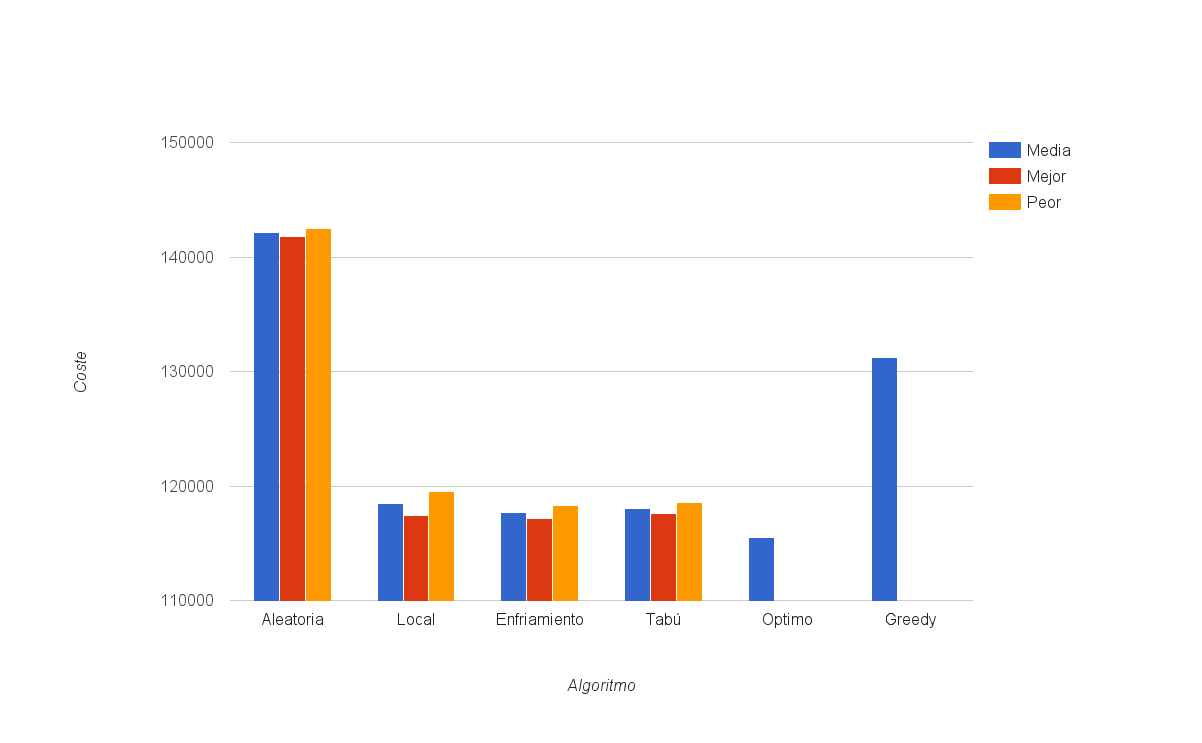
\includegraphics[scale=0.38]{./Grafico90.png}}
\caption{Resultados de los algoritmos para el problema Sko90}
\end{figure}

\begin{table}[H]
\centering
\caption{Resultados globales de los algoritmos para el problema Tai150}
\begin{tabular}{c || r | r | r | r}
Algoritmo 	& Peor & Media & Mejor & Desv. T. \\ \hline
Óptimo 		& - 	& 498896643	&	-	&	-		\\
Greedy 		& - 	& 623469733	&	-	&	-		\\ \hline
B. Aleatoria & 683620162 & 682220716 & 680849383 & \textbf{975284} \\
B. Local & 522055451 & 517687135 & 513041392 & 3103204 \\
Enf. Simu & 524200812 & 516358281 & 513226444 & 3374897 \\
B. Tabú & \quad \textbf{517545690} & \quad \textbf{512865429} & \quad \textbf{510626132} & \quad 2040887 \\
\end{tabular}
\end{table}

\begin{figure}[H]
\center
\centerline{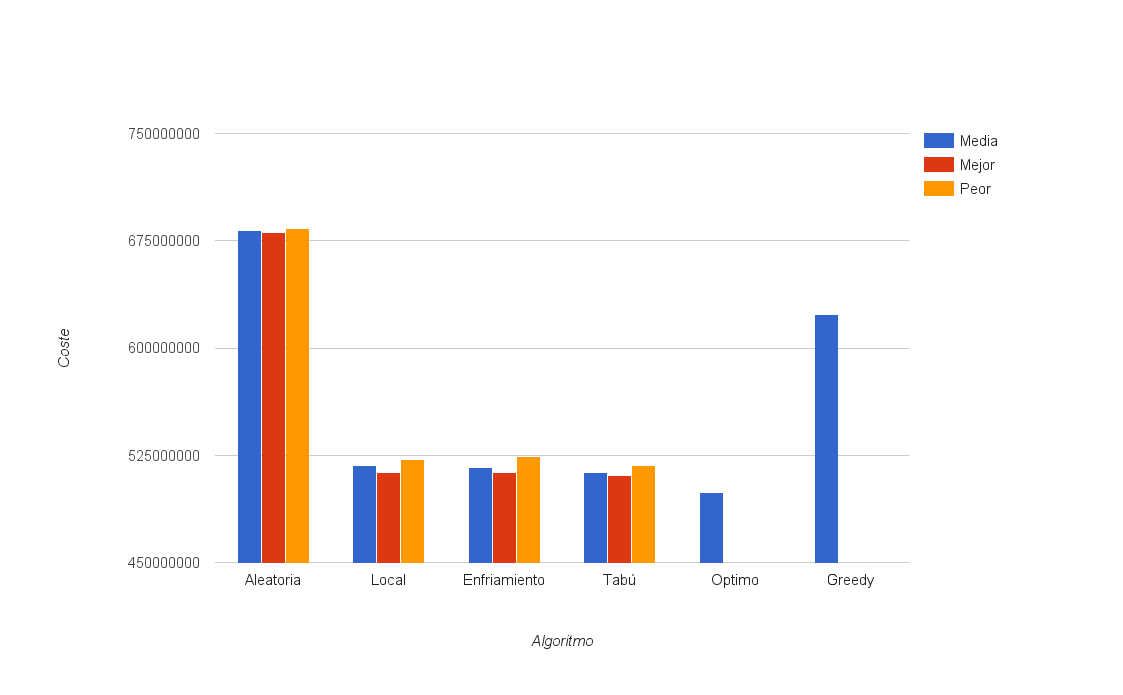
\includegraphics[scale=0.38]{./Grafico150.png}}
\caption{Resultados de los algoritmos para el problema Tai150}
\end{figure}

\section{Análisis y conclusiones}

En general, el algoritmo de Búsqueda Aleatoria obtiene peores resultados que la solución Greedy. Además de tener en todos los casos la desviación típica menor, lo que indica que no solo obtiene malos resultados sino que no suele alejarse de ellos.

Para los tres problemas estudiados el algoritmo de Búsqueda Local obtiene resultados mejores que la solución Greedy y bastante mejores que las soluciones aleatorias, pero tiene una desviación típica alta lo que indica que no es un algoritmo que de resultados sólidos.

Para el problema de tamaño 90 el Enfriamiento simulado obtiene el mejor resultado, seguido muy de cerca por el algoritmo de Búsqueda Tabú que además obtiene el mejor resultado en los otros dos problemas. 

En todos los casos, la desviación típica de los resultados de Búsqueda Tabú es inferior a la de enfriamiento simulado y búsqueda local, lo que indica que es el algoritmo más sólido de todos y tiene más probabilidad de dar una mejor solución en un menor número de ejecuciones.

En cuanto al número de iteraciones, destacar que el algoritmo de Búsqueda Tabú obtiene mejores resultado que el enfriamiento simulado habiendo realizado la mitad de iteraciones y analizando menos vecinos por iteración (40 Tabú frente a 50 enfriamiento).

En general, tanto el Enfriamiento Simulado como la Búsqueda Tabú son buenas opciones frente al resto de algoritmos para enfrentar problemas de búsqueda de grandes dimensiones, sin embargo la mejora de la Búsqueda Tabú sobre el Enfriamiento Simulado no parece demasiado significativa, sobre todo teniendo en cuenta que la implementación del algoritmo Tabú es más compleja.

\end{document}